\documentclass[a4paper,10pt,notitlepage]{article}
\usepackage{ctex,geometry,graphicx,tikz,setspace,paralist,fancyhdr,caption}
\geometry{
	left=1.5cm,
	right=1.5cm,
	top=1.4cm,
	bottom=2cm,}
\newcommand{\rec}{
	\begin{tikzpicture}[remember picture,overlay]
		% 绘制边框
		\draw[line width=1.2pt] ([xshift=0.5cm,yshift=0.5cm] current page.south west) rectangle ([xshift=-0.5cm,yshift=-0.8cm] current page.north east);
	\end{tikzpicture}
	
}
\pagestyle{fancy}
\fancyhf{}
\fancyhead[C]{\rec}  % 在页眉中绘制图形
\fancyhead[L]{模电实验报告}
\fancyhead[R]{实验四 \quad 射极跟随器}
\fancyfoot[C]{\thepage}
\begin{document}
	\large
	\onehalfspacing
	\begin{figure}[h]
		\raggedright
		
\includegraphics{1.png}
	\end{figure}
	\centering
	{\Huge\textbf{模电实验报告}\par}
	\vspace{0.2cm}
	{\huge{实验内容:射极跟随器}\par}
	\raggedright
	\vspace{0.3cm}
	\begin{centering}
		{\large 院系:电子与信息工程学院\hfill 学号:22309080\hfill 审批:\hspace{2cm} \par
			专业:通信工程\hfill 实验人:梁倍铭\hfill 日期:2023年11月9日 \par}
	\end{centering}
	\vspace{0.3cm}
	\section*{一、实验目的}
	\begin{enumerate}
		\item 掌握射极跟随器的特性及测量方法。
		\item 进一步学习放大器各项参数测量方法。
	\end{enumerate}
	\section*{二、原理简介}
	射极跟随器的原理图如图4-1 所示。 它是一个电压串联负反馈放大电路,它具有输
	入电阻高,输出电阻低,电压放大倍数接近于1,输出电压能够在较大范围内跟随输入电
	压作线性变化以及输入、输出信号同相等特点。
	\begin{table}[h]
		\centering
		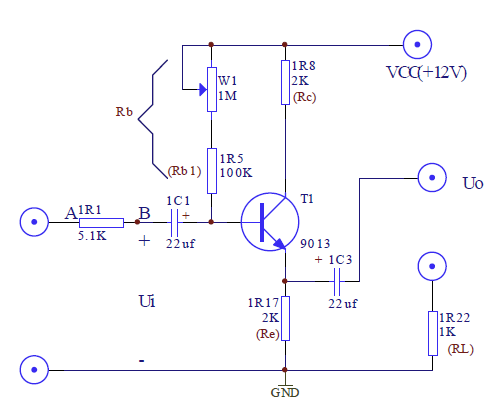
\includegraphics[width=0.6\textwidth]{2.png}
		\caption*{图4-1 射极跟随器电路图}
	\end{table}
	\section*{三、实验器材}
	1、 实验箱 2、数字万用表 3、函数信号发生器 4、交流毫伏表
	5、双踪示波器
	\section*{四、实验步骤和内容}
	\begin{enumerate}
		\item 按图4-1 电路接线。
		\item 直流工作点的调整。\par 
		\qquad 将电源VCC(+l2V)和地(GND)接上,在B 点加f= l kHz 正弦波信号,输出端用示波器
		监视,反复调整W1 及信号源输出幅度,使输出幅度在示波器屏幕上得到一个最大不失真
		波形,然后断开输入信号,用万用表测量晶体管各极对地的电位,即为该放大器静态工作
		点,将所测数据填入表4.1。
	\begin{table}[h]
			\centering
			\begin{tabular}{|c|c|c|c|c|}
				\hline
				& $V_e(V)$ & $V_b(V)$ & $V_c(V)$ & $I_c=V_e/R_e$ \\
				\hline
				仿真 & 6.02531 & 6.68479 & 6.08098 & 3.01mI \\
				\hline
				实验 & 3.067 & 3.627 & 8.943 & 1.534mI  \\
				\hline
			\end{tabular}
			\caption*{表4-1 }
	\end{table}
	\item 测量电压放大倍数AV\par 
	\qquad 接入负载RL(1R22= lKΩ),在B 点f=lkHz 信号,调输入信号辐度(此时偏置电
	位器W1 不能再旋动),用示波器观察,在输出最大不失真情况下测Ui、Uo 值,将所
	测数据填入表4.2 中。\par 
	\begin{figure}[h]
		\centering
		\begin{tabular}{|c|c|c|c|}
			\hline
			& $V_i(V)$ & $U_o(V)$ & $A_v=U_o/U_i$ \\
			\hline
			仿真 & 2.4 & 2.28 &  0.95 \\
			\hline
			实验 & 2.2 & 2.04 & 0.928  \\
			\hline
		\end{tabular}
		\caption*{表4-2 }
	\end{figure}
	\item 测量输出电阻R0\par 
	\qquad 在B 点加f=lKHZ 正弦波信号,Ui=500mV 左右,接上负载RL=1KΩ 时,用示波器观
	察输出波形,测空载输出电压U0 (RL=∞),有负载输出电压UL (RL=1KΩ)的值。
	将所测数据填入表4-3 中。
	$$R_0=(\frac{U_o}{U_L}-1)R_L$$
	\begin{figure}[h]
		\centering
		\begin{tabular}{|c|c|c|c|}
			\hline
			& $U_o(mV)$ & $U_L(mV)$ & $R_o=(U_o/U_L)-1 \times R_L$ \\
			\hline
			仿真 & 998 & 949 & 51.633 \\
			\hline
			实验 & 482 & 440 & 95.45  \\
			\hline
		\end{tabular}
		\caption*{表4-3}
	\end{figure}
	\item 测量放大器输入电阻Ri(采用换算法)\par 
	\qquad 在输入端串入5.1K 电阻,A 点加入f=lKHZ 的正弦波信号,用示波器观察输出波
	形,并分别测A,B 点对地电位VA 、VB。将测量数据填入表4-4。
	$$R_i=\frac{V_B}{V_A-V_B}R$$
	\begin{figure}[h]
		\centering
		\begin{tabular}{|c|c|c|c|}
			\hline
			& $V_A(V)$ & $U_B(V)$ & $R_i=V_B/(V_A-V_B) \times R$ \\
			\hline
			仿真 & 0.7076 & 0.44769 & 8.78k  \\
			\hline
			实验 & 0.1764 & 0.1708 & 155.55k  \\
			\hline
		\end{tabular}
		\caption*{表4-4 }
	\end{figure}
	\item  测射极跟随器的跟随特性并测量输出电压峰值VOPP 。\par 
	\qquad 接入负载RL=1KΩ,在B 点加入f=lkHz 的正弦信号,逐点增大输入信号幅度Ui,
	用示波器监视输出端,在波形不失真时,测所对应的输出UL 值,计算出AV,并用示波
	器测量输出电压的峰值UOPP。与毫伏表读测的对应输出电压有效值比较。将所测数据
	填入表4.5。\par 
	\begin{figure}[h]
		\begin{minipage}{0.3\textwidth}
			\begin{tabular}{|c|c|c|c|c|}
				\hline
				仿真 & 1 & 2 & 3 & 4 \\
				\hline
				$U_i$ & 100mV & 200mV & 500mV & 800mV  \\
				\hline
				$U_L$ & 29.7mV & 63.5mV & 166.93mV & 270.6mV \\
				\hline
				$U_{opp}$ & 84.5mV & 179mV & 467mV & 756mV \\
				\hline
				$A_v$ & 0.845 & 0.895 & 0.934 & 0.945 \\
				\hline
			\end{tabular}
			\caption*{表4-5-1}
		\end{minipage}
		\hspace{4cm}
		\begin{minipage}{0.3\textwidth}
			\begin{tabular}{|c|c|c|c|c|}
				\hline
				实验 & 1 & 2 & 3 & 4 \\
				\hline
				$U_i$ & 100mV & 200mV & 500mV & 800mV  \\
				\hline
				$U_L$ & 34.0mV & 67.9mV & 170.1mV & 272mV \\
				\hline
				$U_{opp}$ & 94.8mV & 184mV & 468mV & 760.9mV \\
				\hline
				$A_v$ & 0.948 & 0.920 & 0.930 & 0.950 \\
				\hline
			\end{tabular}
			\caption*{表4-5-2}
		\end{minipage}
	\end{figure}
\end{enumerate}
\section*{五、实验总结}
\begin{enumerate}
	\item 射极跟随器的原理及特点 \par 
	\qquad 射极跟随器也就是共集电极放大电路,是一种广泛应用的电路。其主要作用是将交流电流放大,以提高整个放大电路的带负载能力。实际电路中,一般用作输出级或隔离级。\par 
	\qquad 其特点为输入阻抗高,输出阻抗低,因而从信号源索取的电流小而且带负载能力强,所以常用于多级放大电路的输入级和输出级;也可用它连接两电路,减少电路间直接相连所带来的影响,起缓冲作用。\par 
	\item  实验数据的误差分析
	\begin{enumerate}
		\item 关于静态工作点的设置,仿真的结果为6v左右,实际操作时发现6v左右也没有失真,但是通过理论计算得知,6v已经达到饱和区,所以应该调到3v左右。
		\item 关于输出电阻的测量,结果比仿真结果大,比理论结果大,可能的原因是对输入电压和输出电压的读数不准确造成
		\item 对输入电阻的测量,串联51k来测输入电阻,51k电阻的电位差较小,会造成测量结果的不准确。
		\item 对射极跟随器的测量,发现放大倍数偏小,原因主要是波形存在噪声,用示波器光标进行测量时会不准确
	\end{enumerate}
	总之,该次实验中测量还是有许多不同之处的,下次实验需要注意。
\end{enumerate}
\section*{六、预习报告}
预习报告见附录
\end{document}